\documentclass[]{article}

\usepackage[T1]{fontenc}
\usepackage[utf8]{inputenc}
\usepackage[english]{babel}
\usepackage[left=1.5cm,right=1.5cm,top=2cm,bottom=2.5cm]{geometry}

\usepackage[fontsize=13pt]{scrextend}

\renewcommand{\baselinestretch}{1.3}

\usepackage[nooneline]{caption}
\usepackage{subcaption}
\usepackage{indentfirst}
\usepackage{tabularx}
\usepackage{amsmath}
\usepackage{multirow}
\usepackage{hyperref}



\usepackage{fancyhdr}


\setlength{\headheight}{15mm}


\usepackage[pdftex]{graphicx}
\graphicspath{{../Report/img/}{img/}}

\pagestyle{fancy}
\lhead{\textbf{\normalsize Project 2}}
\rhead{\textbf{\normalsize Author: }\normalsize Maksim Kiryakin}



\begin{document}

{
	\Large
	\href{https://github.com/MaximKiryakin/quant-finance-projects/tree/main/volatility-har-garch}{Project repository}.
}

\section{Problem statement}


The goal of this work is to forecast the volatility of a chosen asset using GARCH and HAR models.

[Bollerslev, 1986]: the \textbf{GARCH(p, q)} model:

$$\varepsilon_t = \nu_t \sqrt{h_t}$$
$$h_t = a_0 + a_1\varepsilon_{t-1}^2 + ... + a_p\varepsilon_{t-p}^2 + b_1 h_{t-1} + ... + b_q h_{t-q}$$

where $\nu_t \sim iid$, $\mathbf{E}(\nu_t) = 0$, $\mathbf{D}(\nu_t) = 1$, and $a$, $b$ are parameters.

\textbf{Realized volatility}

$RV_t$ --- the realized volatility for period $t$ (usually a day) --- is given by the following formula:

$$RV_{t} = \sqrt{\sum_{j}r_{t, j}^2}$$


where $r_{t, j} = \log{p_{t, j}} - \log{p_{t, j-1}}$ is the log-return for intraday period $j$ of day $t$, and $p_{t, j}$ is the asset price on day $t$ in intraday period $j$.


[Corsi, 2009]: the \textbf{HAR(w, m)} model:

$$RV_t = \beta_0 + \beta_1 RV_{t-1} + \beta_2 RV_{t-1}^w + \beta_3 RV_{t-1}^m + \varepsilon_t$$

where:

$RV_{t}^w = \frac{1}{w}\sum_{j=0}^{w-1}RV_{t-j}$ is the average realized volatility over a week;
$RV_{t}^m = \frac{1}{m}\sum_{j=0}^{m-1}RV_{t-j}$ is the average realized volatility over a month; $w$ is the number of trading days in a week; $m$ is the number of trading days in a month.



\section{Data}


The underlying asset is Sberbank stock, over the period from January 3, 2020 to November 29, 2024. Sberbank (ticker SBER) is a Russian financial conglomerate, the largest universal bank in Russia and Eastern Europe. Its shares trade on the Moscow Exchange, are part of the ``blue chips'' of the Russian stock market, and reflect its dynamics well ($\beta = 0.82$ as of December 1, 2024).

The project was carried out using two languages: Python and R. The former was used for the initial processing and analysis of the quote data, the latter for building and estimating the models.
The data were downloaded using the getSymbols function of the R package rusquant. The data frequency is 5 minutes.
The resulting data frame contained 95,868 records. Figures $\ref{price}$ and $\ref{vol}$ show the Sberbank stock price over the specified period and its return, respectively.

\begin{figure}[h!]
	\centering
	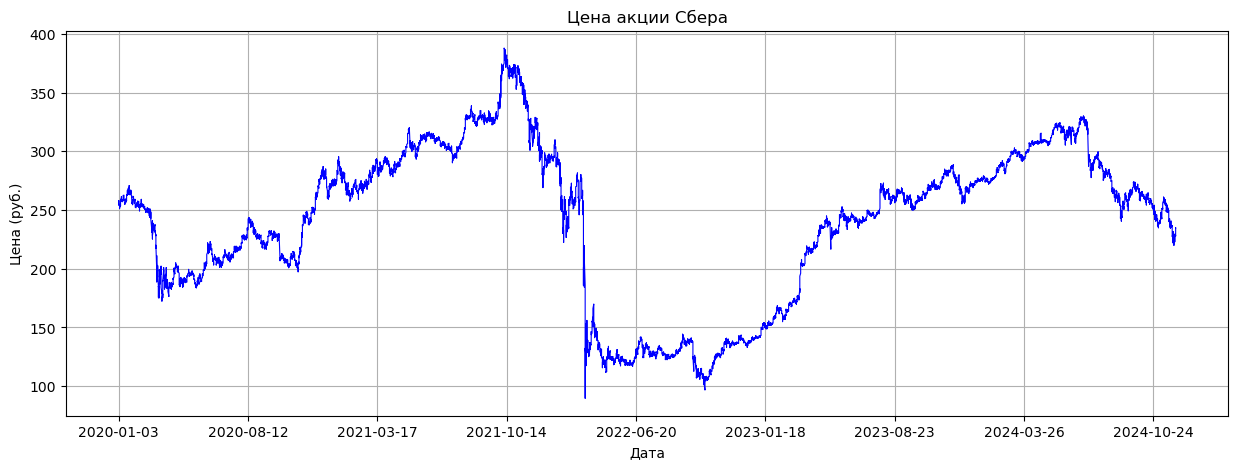
\includegraphics[width=1.\textwidth]{price.png}
	\caption{Sberbank closing stock price over 2020-01-03 to 2024-11-28.}
	\label{price}
\end{figure}

\begin{figure}[h!]
	\centering
	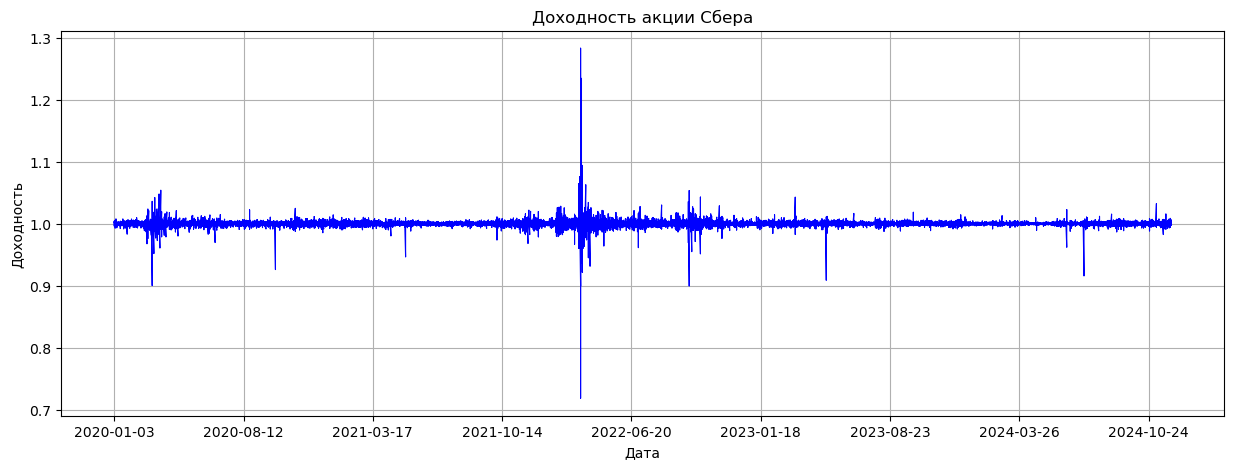
\includegraphics[width=1.\textwidth]{vol.png}
	\caption{Sberbank stock return dynamics over 2020-01-03 to 2024-11-28.}
	\label{vol}
\end{figure}

Figure $\ref{vol}$ shows that the data exhibit volatility clustering. In addition, gaps were found in the data for days with no trading. These periods were excluded during model training.

Furthermore, Figure $\ref{hist}$ shows a histogram of the returns with a kernel density estimate. For comparison, the density of the normal distribution is also added. The plot shows that the actual density estimate differs from the normal one. Based on these distributions, one can expect that models with normally distributed residuals will perform worse than those that assume, for example, a Student's $t$-distribution.

\begin{figure}[h!]
	\centering
	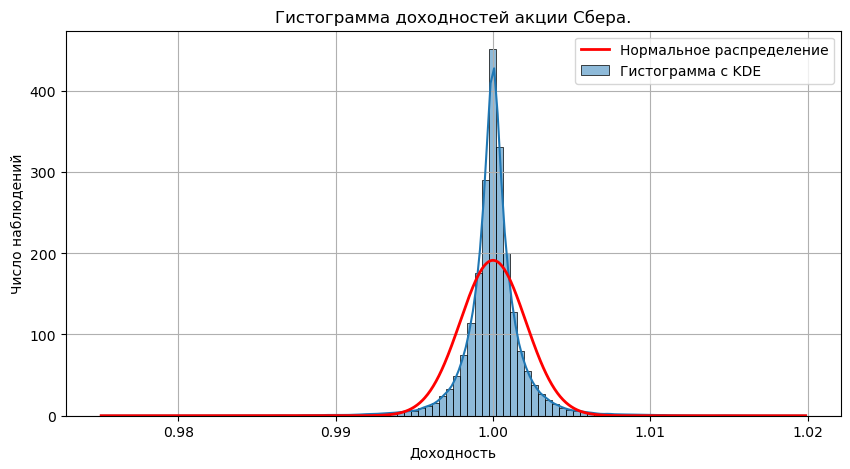
\includegraphics[width=1.\textwidth]{hist.png}
	\caption{Histogram of Sberbank stock returns over 2020-01-03 to 2024-11-28.}
	\label{hist}
\end{figure}




\section{Methodology}
\subsection{Selected models and their specification}


The comparison includes the following five GARCH models.

1. Standard GARCH(p, q)
$$\varepsilon_t = \nu_t \sqrt{h_t}$$
$$h_t = a_0 + a_1\varepsilon_{t-1}^2 + ... + a_p\varepsilon_{t-p}^2 + b_1 h_{t-1} + ... + b_q h_{t-q}$$

here and below: $h_t$ is the conditional variance at time $t$; $a$, $b$ are parameters estimated by maximum likelihood; $\nu_t \sim iid$, $\mathbf{E}(\nu_t) = 0$, $\mathbf{D}(\nu_t) = 1$.

2. Exponential GARCH (EGARCH)
$$\ln{h_t} = a_0 + a_1(|\varepsilon_{t-1}| - E(|\varepsilon_{t-1}|)|) + \theta\varepsilon_{t-1} + b\ln{h_{t-1}}$$

3. Integrated GARCH (iGARCH)

An additional constraint is imposed on the coefficients:

$$\sum_{i=1}^{p} a_i + \sum_{i=1}^{q} b_i = 1$$

4. Threshold GARCH (TGARCH)
$$\sqrt{h_t} = a_0 + a_1^{+}\varepsilon_{t-1}^{+} + a_1^{-}\varepsilon_{t-1}^{-} + b_1\sqrt{h_{t-1}}$$

$$
	\varepsilon_{t-1}^{+} =
	\begin{cases}
		\varepsilon_{t-1}, & \text{if} \ \varepsilon_{t-1} > 0 \\
		0, & \text{otherwise}
	\end{cases}
$$

$$
	\varepsilon_{t-1}^{-} =
	\begin{cases}
		\varepsilon_{t-1}, & \text{if} \ \varepsilon_{t-1} < 0 \\
		0, & \text{otherwise}
	\end{cases}
$$

5. Nonlinear/asymmetric NAGARCH
$$h_t = a_0 + a_1(\varepsilon_{t-1} - \theta\sqrt{h_{t-1}})^2 + b_1 h_{t-1}, \quad \theta > 0$$


Each of the GARCH-type models above is estimated with each of three conditional error-distribution models:

1. Standard normal distribution (norm) with density

\begin{equation}
	\varphi(x) = \frac{1}{\sqrt{2\pi}} e^{-\frac{x^2}{2}}.
\end{equation}

2. Skew-normal distribution (snorm)

\begin{equation}
	f(x) = 2\varphi(x)\Phi(\alpha x),
\end{equation}

where \(\varphi(x)\) and \(\Phi(x)\) are the probability density function and the cumulative distribution function of a standard normal random variable.

3. Skewed Student's \(t\)-distribution (\textit{sstd})

$$f(z, \xi) = \frac{2}{\xi + \xi^{-1}} \left[ f(\xi z) I(-z) + f(z/\xi) I(z) \right]$$

where \(f(x)\) is the Student's $t$ density and
$$I(z) =
\begin{cases}
	1, & z > 0, \\
	0, & z \leq 0.
\end{cases}
$$

In addition to the GARCH family, the following three HAR models were considered:

1. HAR model

$$RV_t = \beta_0 + \beta_1 RV_{t-1} + \beta_2 RV_{t-1}^w + \beta_3 RV_{t-1}^m + \varepsilon_t$$

where:
\begin{itemize}

	\item $RV_t$ --- realized volatility for period $t$

	\item $r_{t, j} = \log{p_{t, j}} - \log{p_{t, j-1}}$ --- log-return for intraday period $j$ of day $t$

	\item $RV_{t} = \sqrt{\sum_{j}r_{t, j}^2}$

	\item $RV_{t}^w = \frac{1}{w}\sum_{j=0}^{w-1}RV_{t-j}$

	\item $RV_{t}^m = \frac{1}{m}\sum_{j=0}^{m-1}RV_{t-j}$

\end{itemize}

2. HARQ model:
$$RV_t = \beta_0 + \beta_1 RV_{t-1} + \beta_2 RV_{t-1}^w + \beta_3 RV_{t-1}^m + \beta_{1Q}\sqrt{RQ_{t-1}}RV_{t-1} + \beta_{2Q}\sqrt{RQ_{t-1}^w} RV_{t-1}^w  + \beta_{3Q}\sqrt{RQ_{t-1}^m}RV_{t-1}^m + \varepsilon_{t}$$

where $RV_t$ is realized volatility for period $t$; $r_{t, j} = \log{p_{t, j}} - \log{p_{t, j-1}}$ is the log-return for intraday period $j$ of day $t$; $RV_{t} = \sqrt{\sum_{j}r_{t, j}^2}$; $RV_{t}^w = \frac{1}{w}\sum_{j=0}^{w-1}RV_{t-j}$; $RV_{t}^m = \frac{1}{m}\sum_{j=0}^{m-1}RV_{t-j}$; $RQ_{t} = \sum_{j=0}r_{tj}^4$ --- realized quarticity.

3. HARJ model:

$$RV_t = \beta_0 + \beta_1 RV_{t-1} + \beta_2 RV_{t-1}^w + \beta_3 RV_{t-1}^m + \beta_{4}J_t + \beta_5 J_t^w + \beta_6 J_t^m + \varepsilon_{t}$$

where:

$BPV_t = \sum_{j=1}r_{t, j}r_{t, j-1}$ --- realized bipower variation, which allows accounting for the trend in the data.

$Jump: J = \max(RV_t - BPV_t, 0)$


\subsection{Comparison of GARCH models}


The models were evaluated using three metrics: MSE, MAE, MAPE. For the GARCH family, GARCH(1, 1)-norm was used as the naive forecast. Model validation was performed on Sberbank stock prices over the interval 2024-10-21 to 2024-11-29. An expanding window was used to compute the metrics. Predictions were made one day ahead. The target variable was the realized volatility on each day.
The R library rugarch was used for forecasting.

It was found that validating a GARCH-family model on a home PC took more than an hour, which made expanding-window validation of all models infeasible. Moreover, convergence problems sometimes arose and the main model-search loop had to be restarted. Reducing the number of observations was not appropriate, since training this class of models requires tens of thousands of observations.

Therefore, an alternative model-comparison approach was proposed. Models were ranked according to the AIC and BIC information criteria, and the best models were evaluated on an expanding window.




\begin{table}[h!]
	\centering
	\caption{Information-criterion values for various GARCH models.}
	\begin{tabularx}{\textwidth}{|X|X|X|l|l|l|}
		\hline
		                    	& AIC        & BIC        & MAE          & MSE             & MAPE    \\ \hline
		GARCH(1, 1)-norm        & -9.935168  & -9.934575  & 0.02184 &  0.000488   & 0.995   \\ \hline
		TGARCH(1, 1)-sstd       & -10.36761  & -10.36682  &0.02183  &0.000487     &0.994   \\ \hline
		     ...    &  &   &&&    \\ \hline
		NAGARCH(1, 1)-norm      & -9.937876  & -9.860202  &&&    \\ \hline


	\end{tabularx}
	\label{tab:1}
\end{table}



As expected, the experiments showed that the skewed Student's distribution yields better information-criterion values than the other distributions. QQ-plots for the normal and skewed distributions are shown in Figures $\ref{badQQ}$ and $\ref{goodQQ}$, respectively.


\begin{figure}[h!]
	\centering
	\begin{subfigure}{0.49\textwidth}
		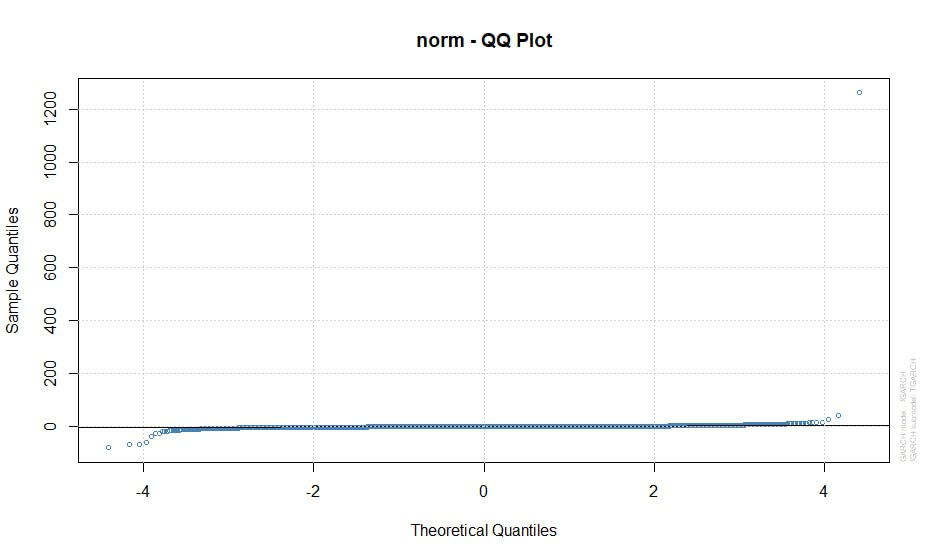
\includegraphics[width=\linewidth]{badQQ.jpg}
		\caption{QQ-plot for the TGARCH model (normal error distribution).}
		\label{badQQ}
	\end{subfigure}
	\hfill
	\begin{subfigure}{0.49\textwidth}
		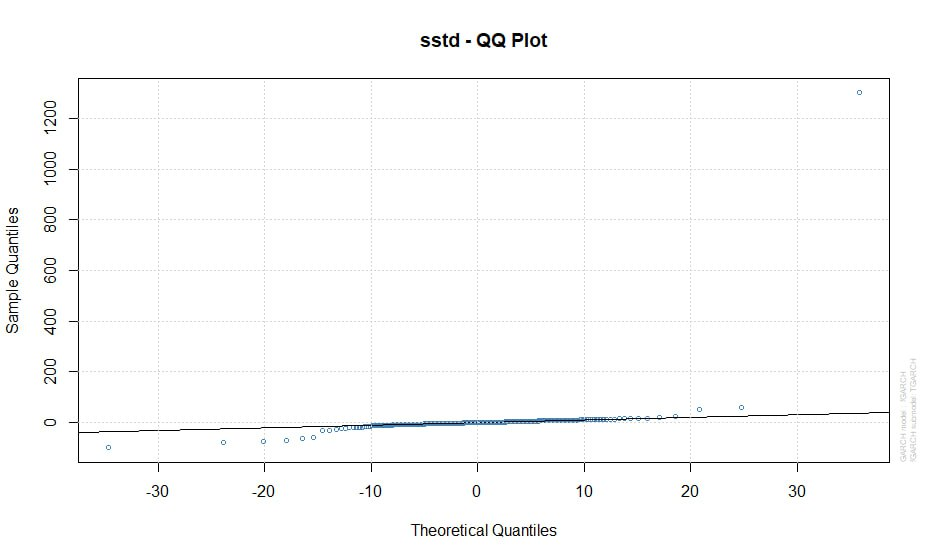
\includegraphics[width=\linewidth]{goodQQ.jpg}
		\caption{QQ-plot for the TGARCH model (skewed Student's error distribution).}
		\label{goodQQ}
	\end{subfigure}
\end{figure}




Figures $\ref{normNews}$ and $\ref{skewNews}$ show the news-impact curves on volatility. For TGARCH the curve is asymmetric, indicating that negative news affects volatility more strongly than positive news.

\begin{figure}[h!]
	\centering
	\begin{subfigure}{0.49\textwidth}
		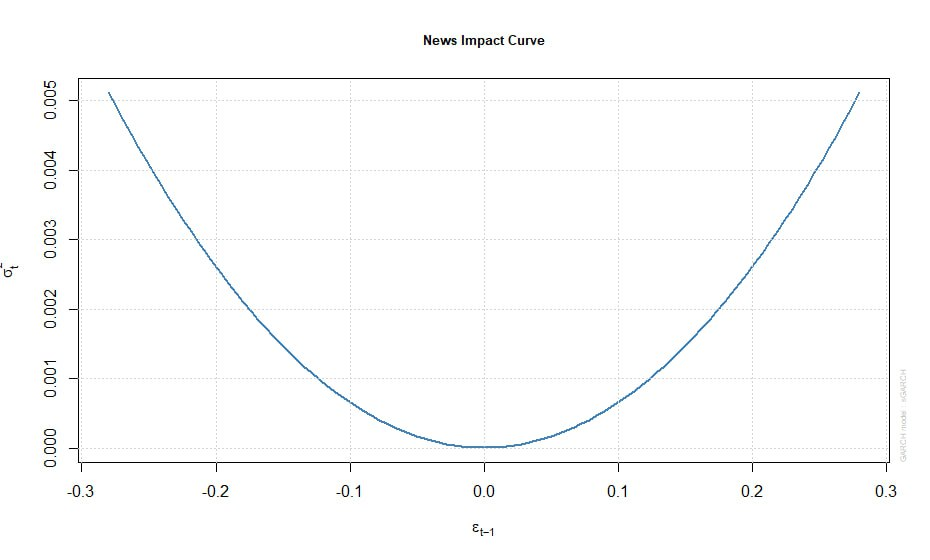
\includegraphics[width=\linewidth]{normNews.jpg}
		\caption{Impact of positive and negative news on volatility for GARCH.}
		\label{normNews}
	\end{subfigure}
	\hfill
	\begin{subfigure}{0.49\textwidth}
		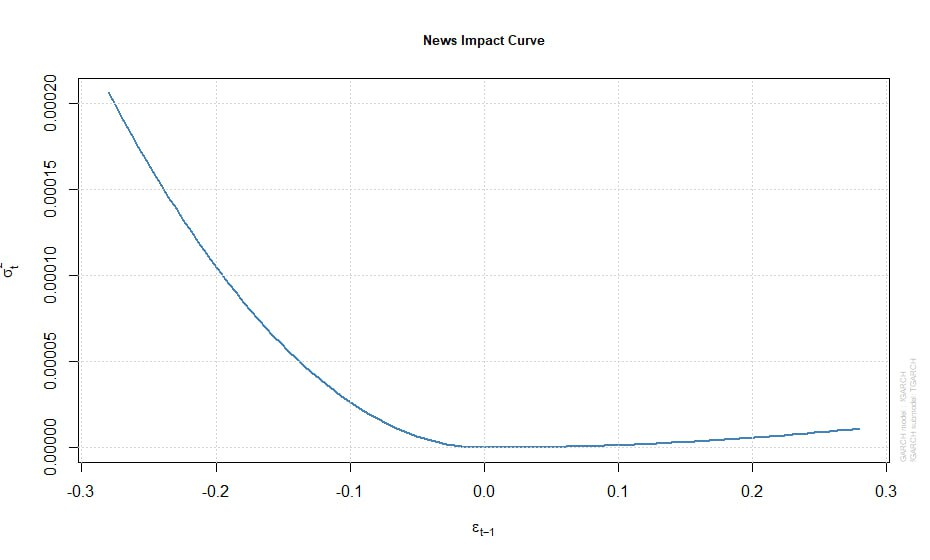
\includegraphics[width=\linewidth]{skewNews.jpg}
		\caption{Impact of positive and negative news on volatility for TGARCH.}
		\label{skewNews}
	\end{subfigure}
	\label{fig:both_images}
\end{figure}

The experiments also showed that because the model poorly captures the volatility dynamics one day ahead (in our case more than 100 five-minute intervals), all results turned out roughly similar. Running an experiment forecasting 5 minutes ahead at each step would require a supercomputer, but the forecast accuracy should then increase substantially. Table $\ref{tab:1}$ shows that the best model by information criteria was TGARCH(1,1)-sstd, but its advantage over the naive GARCH(1, 1)-norm forecast is negligible under expanding-window validation.


\subsection{Comparison of HAR models}

The HAR-model forecasts used the same data as the GARCH models. The forecast was made over the same horizon, which allows comparing the two approaches. The HARForecast function from the HARModel library was used. The HAR-model results are given in Table $\ref{tab:2}$. The simple HAR model performed best on the chosen validation interval.

\begin{table}[h!]
	\centering
	\caption{Metric values for various HAR models.}
	\begin{tabularx}{\textwidth}{|X|X|X|X|}
		\hline
		       &   MAE        & MSE       & MAPE    \\ \hline
		HAR    & 0.002981667  & 1.768148e-05  & 0.198    \\ \hline
		HARQ   & 0.004232569  & 3.178277e-05  & 0.286    \\ \hline
		HARJ   & 0.003746625  & 2.624049e-05  & 0.253    \\ \hline
	\end{tabularx}
	\label{tab:2}
\end{table}

Figures $\ref{HAR}$ and $\ref{HARQ}$ show the 30-day-ahead volatility forecasts for the HAR and HARQ models, respectively.


\begin{figure}[h!]
	\centering
	\begin{subfigure}{0.49\textwidth}
		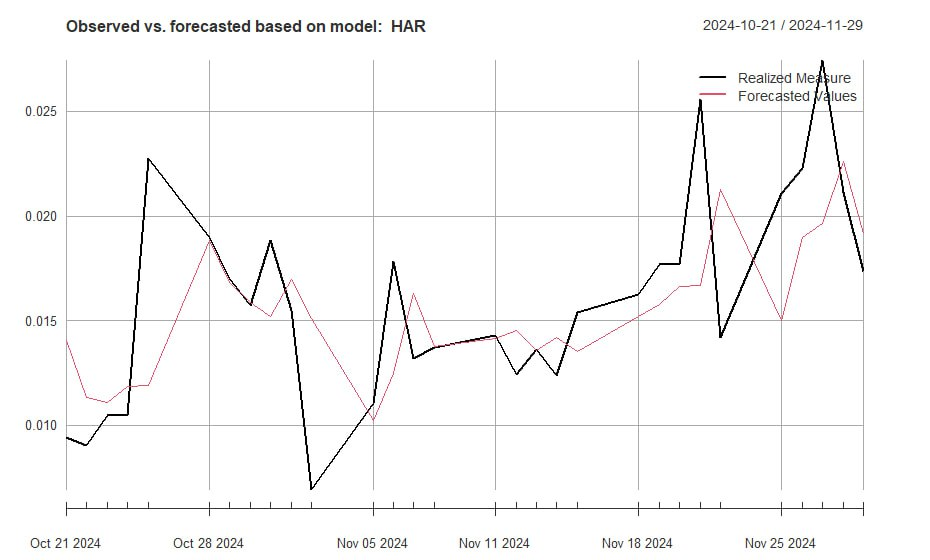
\includegraphics[width=\linewidth]{HAR.jpg}
		\caption{30-day volatility forecast by the HAR model.}
		\label{HAR}
	\end{subfigure}
	\hfill
	\begin{subfigure}{0.49\textwidth}
		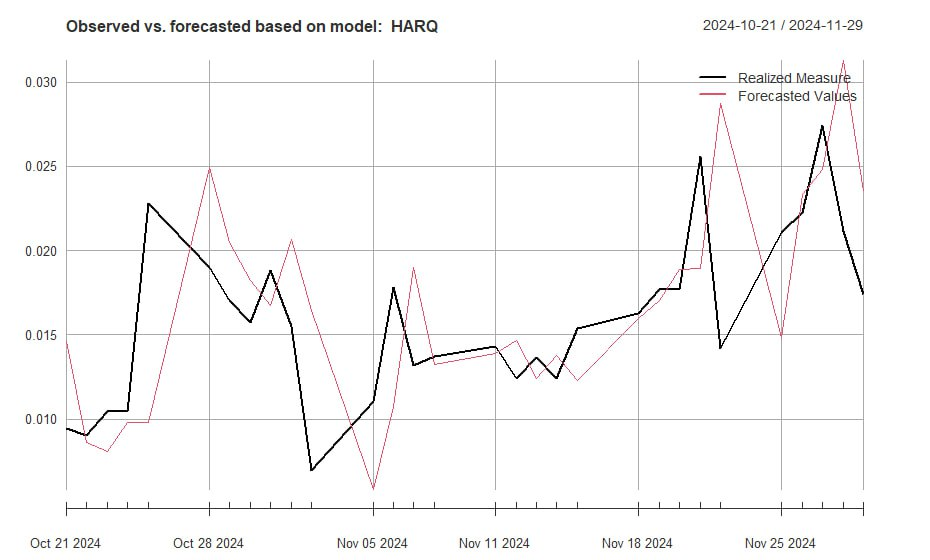
\includegraphics[width=\linewidth]{HARQ.jpg}
		\caption{30-day volatility forecast by the HARQ model.}
		\label{HARQ}
	\end{subfigure}
	\label{fig:both_images}
\end{figure}


\subsection{Comparison of HAR models on high-volatility data}

In addition to varying the model specifications, the models were also tested over different time intervals. The second interval considered was from January 1, 2017 to March 25, 2020. During this period the Russian stock market was extremely unstable due to the spread of COVID.

HAR models were chosen for these tests, since they outperformed GARCH models in the initial testing. Moreover, their training is an order of magnitude faster, which was very important here. The forecast was again performed with an expanding window, one day ahead. The results are given in Table $\ref{tab:3}$.


\begin{table}[h!]
	\centering
	\caption{Metric values for various HAR models on high-volatility data.}
	\begin{tabularx}{\textwidth}{|X|X|X|X|}
		\hline
		       &   MAE   & MSE      & MAPE     \\ \hline
		HAR    & 0.0088  & 0.00018  & 0.300    \\ \hline
		HARQ   & 0.0090  & 0.00019  & 0.305    \\ \hline
		HARJ   & 0.0099  & 0.00021  & 0.324    \\ \hline
	\end{tabularx}
	\label{tab:3}
\end{table}

The table shows that on volatile data the HAR and HARQ forecasts are very close ($\frac{MAE(HARQ)}{MAE(HAR)} = 1.034841$), which does not allow concluding with certainty that the former model is better and requires more detailed tests.

Figures $\ref{HARVol}$ and $\ref{HARQVol}$ show the HAR and HARQ forecasts on volatile data.


\begin{figure}[h!]
	\centering
	\begin{subfigure}{0.49\textwidth}
		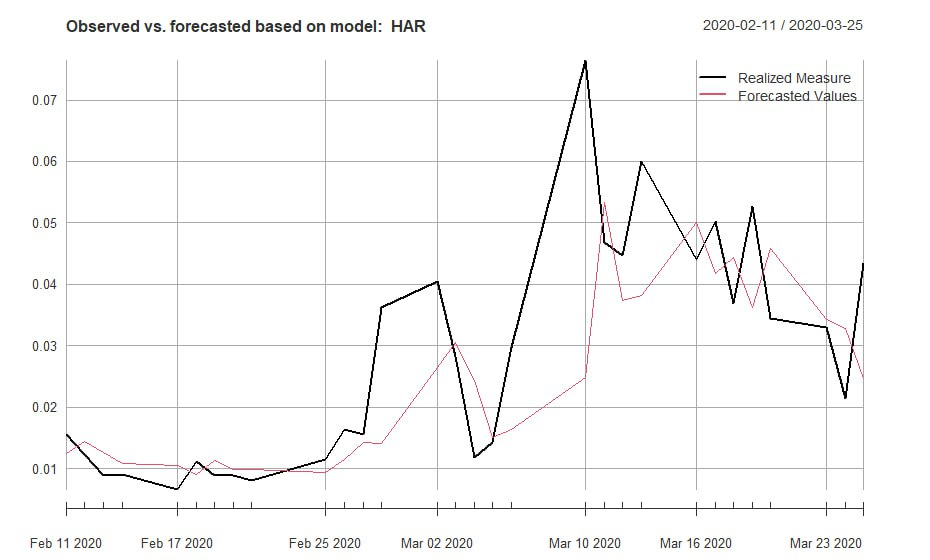
\includegraphics[width=\linewidth]{HARVol.jpg}
		\caption{HAR-model forecast on volatile data.}
		\label{HARVol}
	\end{subfigure}
	\hfill
	\begin{subfigure}{0.49\textwidth}
		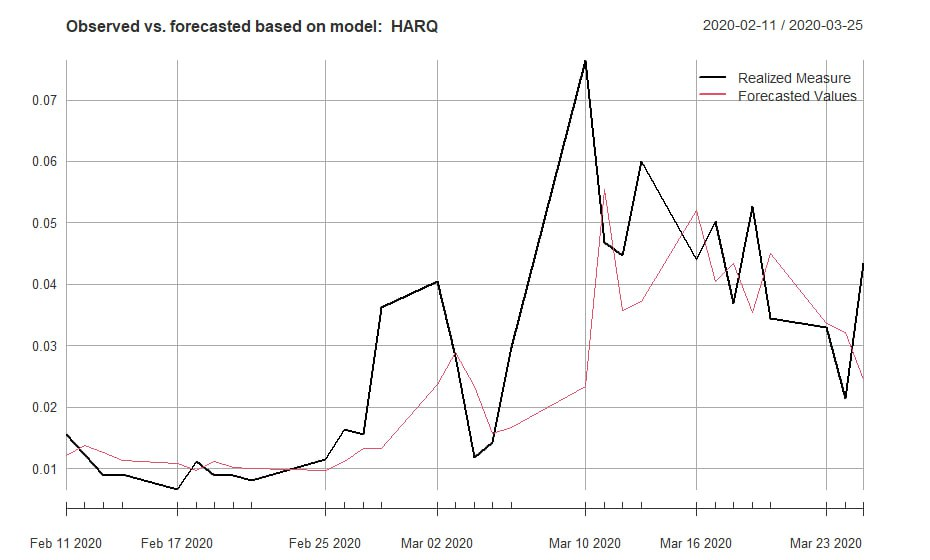
\includegraphics[width=\linewidth]{HARQVol.jpg}
		\caption{HARQ-model forecast on volatile data.}
		\label{HARQVol}
	\end{subfigure}
\end{figure}


\section{Conclusion}

This work compared two classes of volatility-prediction models, HAR and GARCH. The underlying asset was Sberbank stock. Two time intervals were considered: from January 3, 2020 to November 29, 2024, and from January 1, 2017 to March 25, 2020. The second interval was considered only for HAR models and was treated as more volatile than the first.

The comparison included the following GARCH-family models: GARCH, EGARCH, NAGARCH, TGARCH, IGARCH; and the following HAR-family models: HAR, HARQ, HARJ.
On the first dataset, among the GARCH models TGARCH(1, 1)-sstd performed best, and among the HAR family the plain HAR model. On highly volatile data the HAR and HARQ results are comparable. The results of the selected algorithms are given in Table $\ref{tab:4}$.

\begin{table}[h!]
	\centering
	\caption{Metric values of the selected volatility-prediction models.}
	\begin{tabularx}{\textwidth}{|X|X|X|X|l|}
		\hline
								  & Model            &   MAE   & MSE     & MAPE     \\ \hline
		                          & TGARCH(1,1)-sstd & $2.2\cdot10^{-2}$ & $4.9\cdot10^{-4}$  & 0.994    \\ \cline{2-5}
		\centering{Period}        & GARCH(1,1)-norm  & $2.2\cdot10^{-2}$ & $4.9\cdot10^{-4}$  & 0.995    \\ \cline{2-5}
    	\centering{2020-01-03}    & HAR              & $3.0\cdot10^{-3}$ & $1.8\cdot10^{-5}$  & 0.198    \\ \cline{2-5}
    	\centering{to 2024-11-29} & HARQ             & $4.2\cdot10^{-3}$ & $3.2\cdot10^{-5}$  & 0.286    \\ \cline{2-5}
    	                          & HARJ             & $3.7\cdot10^{-3}$ & $2.6\cdot10^{-5}$  & 0.253    \\ \cline{2-5}
    	                          & Naive            & $3.3\cdot10^{-3}$ & $2.7\cdot10^{-5}$  & 0.221    \\ \hline
		\centering{Period}        & HAR              & $8.8\cdot10^{-3}$ & $1.8\cdot10^{-4}$  & 0.300    \\ \cline{2-5}
		\centering{2017-01-01}    & HARQ             & $9.0\cdot10^{-3}$ & $1.9\cdot10^{-4}$  & 0.305    \\ \cline{2-5}
		\centering{to 2020-03-25} & HARJ             & $9.9\cdot10^{-3}$ & $2.1\cdot10^{-4}$  & 0.324    \\ \cline{2-5}
		                   & Naive            & $1.4\cdot10^{-2}$ & $3.3\cdot10^{-4}$  & 0.868    \\ \cline{2-5}
		\hline
	\end{tabularx}
	\label{tab:4}
\end{table}

The experiments established that the HAR-model forecast is much more accurate than GARCH. However, the quality of the GARCH model could be improved by forecasting not one day ahead but, for example, 5 minutes ahead.

In addition, the table includes the metric values of a naive realized-volatility forecast, taken as the average over the last 3 days. The experiments show that for relatively non-volatile data the naive forecast even outperformed the HAR models on the MAPE metric. On volatile data, however, the naive forecast loses to the HAR models. Based on these results, one can speak of the effectiveness of HAR models on volatile data.

\end{document}
